\iffalse Do not add content to this file, this file will be used to compile the files in this folder. \fi
\documentclass{article}
\usepackage{hyperref}
\usepackage{graphicx}
\usepackage{float}
\hypersetup{
    colorlinks,
    citecolor=black,
    filecolor=black,
    linkcolor=black,
    urlcolor=black
}

\makeatletter
\renewcommand\paragraph{\@startsection{paragraph}{4}{\z@}%
            {-2.5ex\@plus -1ex \@minus -.25ex}%
            {1.25ex \@plus .25ex}%
            {\normalfont\normalsize\bfseries}}
\makeatother
\setcounter{secnumdepth}{4} % how many sectioning levels to assign numbers to
\setcounter{tocdepth}{4}    % how many sectioning levels to show in ToC

\begin{document}
		\begin{figure}[t]
			\centering
			
\includegraphics[width=350px]{UP_Logo.PNG}
		\end{figure}
			\title{COS 301 Software Engineering\\ Testing the implementation of Broadsword: Navigation}
\maketitle
		\begin{center}
			\textbf{\newline Longsword Navigation} \\
		\end{center}
			
				
		\begin{flushright} \large
			Duart Breedt - u15054692\\			
			Marin Peroski - u13242475\\
			Nathan Ngobale -  u15110045\\
			Azhar Patel - u15052592\\
			Duart Breedt - u15054692\\
			Matthew Perry - u13017030\\
			Neo Thokoa - u14163285\\
		\end{flushright}
		
		
		
		
		GitHub Repository: \href{https://github.com/perrymatthew/cos301_Longsword_Navigation}\\
		\url{https://github.com/perrymatthew/cos301_Longsword_Navigation}
	

\clearpage
\tableofcontents
\clearpage

\section{Introduction}

\clearpage

\section{Non-Functional Requirements}
	\begin{itemize}
	
	\item \textbf{Maintainability:}\\Coding standards were upheld and the code was well documented. However, the lack of compartmentalization of functionality may prove problematic when  removing, adding, or editing program features. Furthermore, the location data is kept in a single file with the program therefore if a location should be added it cannot be added with a database query but had to be done manually \textbf{Mark: 6/10}
	\item \textbf{Scalability:}\\MongoDB as a choice of database management is favourable especially with regards scalability. However, the location data is not stored in a MongoDB database but rather in the same navigationLocal.js file as the entire program. This will cause a bottleneck when the amount of location data is increased. \textbf{Mark: 7/10}
	\item \textbf{Accessibility:}\\All functions allowed other modules to request information as well as get a result returned if needed. The scope of the functions were adequate, allowing other modules to call needed functions. However, the scope was broad and did allow access functions which other modules should not have access to. \textbf{Mark: 8/10}
	
\end{itemize}
\clearpage
	
\section{Test Models}
	\iffalse Do not add content to this file, this file will be used to compile the files in this folder. \fi
\clearpage

\section{Service Contracts}
	\begin{itemize}
	
\item \textbf{Save User Route:}\\Coding standards were upheld and the code was well documented. However, the lack of compartmentalization of functionality may prove problematic when  removing, adding, or editing program features. Furthermore, the location data is kept in a single file with the program therefore if a location should be added it cannot be added with a database query but had to be done manually.\\
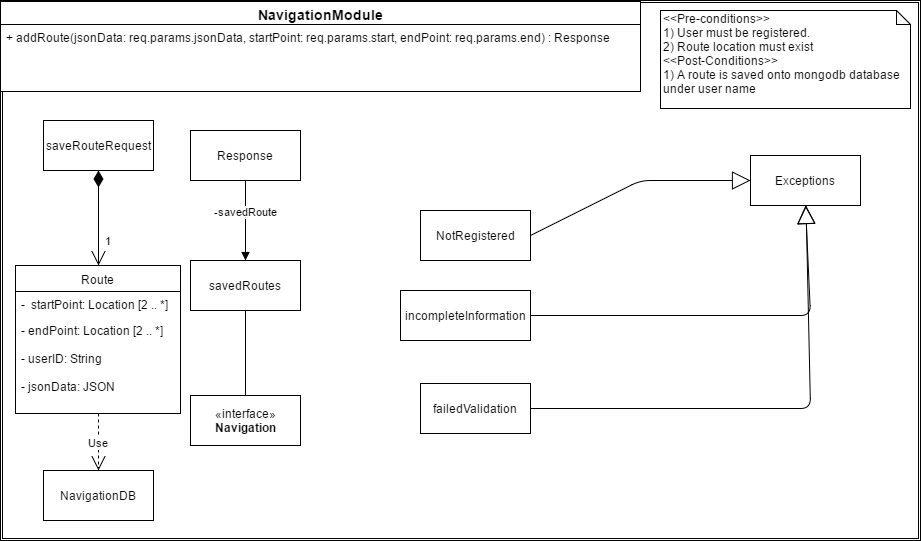
\includegraphics[scale=0.5]{SaveRoute.png}
\caption{Service Contract: Save User Preference}
	\textbf{Mark: 6/10}
\item \textbf{Save User Preference:}\\MongoDB as a choice of database management is favourable especially with regards scalability. However, the location data is not stored in a MongoDB database but rather in the same navigationLocal.js file as the entire program. This will cause a bottleneck when the amount of location data is increased.\\
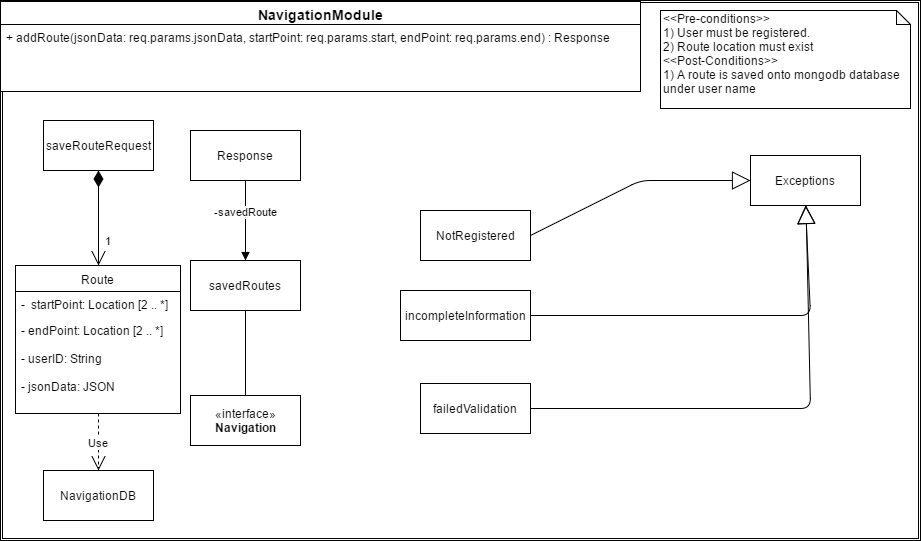
\includegraphics[scale=0.5]{SaveRoute.png}
\caption{Service Contract: Save User Preference}
	\textbf{Mark: 7/10}
\item \textbf{Cache Routes:}\\MongoDB as a choice of database management is favourable especially with regards scalability. However, the location data is not stored in a MongoDB database but rather in the same navigationLocal.js file as the entire program. This will cause a bottleneck when the amount of location data is increased.\\
	\textbf{Mark: 7/10}
	
\end{itemize}


\end{document}